
%\xymatrix{
%	A \ar[r]^f \ar[dr]_g & B \ar[d]^h \\
%	& C 
%} $\longrightarrow$  \xymatrix{
%A \ar[r]^f \ar[dr]_g & B \ar[d]^h \\
%& C 
%}



%$$
%\xymatrix{
%	A \ar[rr]^f \ar[ddrr]_{f\circ g}& & B \ar[dd]^g &          &  & F(A) \ar[rr]^{F(f)} \ar[ddrr]_{F(g\circ f)}& & F(B) \ar[dd]^{F(g)} \\
%	                              & &             & \ar[rr]^F &  &                                            & &\\
%                                  & & C           &          &  &                                            & &  C'
%} $$       \ar@(dr,dl)[]



\section{Functores}

\begin{definicion}\label{ppoiujhgf}
	\upshape{
		Dadas dos categorías $\mathcal{C}$ y $\mathcal{D}$, un \textit{functor} de $\mathcal{C}$ a $\mathcal{D}$ es una asignación $F : \mathcal{C} \to \mathcal{D}$ que consiste en:
		
		\begin{enumerate}
			\item Una función entre las clases de objetos:
			\begin{align*}
				\mathrm{Ob}(\mathcal{C}) &\longrightarrow \mathrm{Ob}(\mathcal{D}) \\
				A &\longmapsto F(A)
			\end{align*}
			
			\item Para cada par de objetos $A, B \in \mathrm{Ob}(\mathcal{C})$, una función entre las clases de morfismos:
			\begin{align*}
				\mathrm{Hom}_{\mathcal{C}}(A, B) &\longrightarrow \mathrm{Hom}_{\mathcal{D}}\left(F(A), F(B)\right) \\
				f &\longmapsto F(f)
			\end{align*}
			que respeta:
			\begin{itemize}
				\item La identidad: $F(\mathrm{id}_A) = \mathrm{id}_{F(A)}$ para todo $A \in \mathrm{Ob}(\mathcal{C})$.
				
				\item La composición: Si $f \in \mathrm{Hom}_{\mathcal{C}}(A, B)$ y $g \in \mathrm{Hom}_{\mathcal{C}}(B, C)$, entonces
				$$
				F(g \circ f) = F(g) \circ F(f).
				$$
				Esto significa que a un diagrama conmutativo, el functor $F$ le asigna otro diagrama también conmutativo.
				
				$$
					{\Large
						\xymatrix{
								A \ar[rr]^f \ar[ddrr]_{f\circ g}& & B \ar[dd]^g &          &  & F(A) \ar[rr]^{F(f)} \ar[ddrr]_{F(g\circ f)}& & F(B) \ar[dd]^{F(g)} \\
								                              & &             & \ar[rr]^F &  &                                            & &\\
							                                & & C           &          &  &                                            & &  F(C)
							}
					} 
				$$
				
			\end{itemize}
		\end{enumerate} 
	}
\end{definicion}

\begin{observacion}
	\upshape{
		Las categorías se relacionan entre sí mediante functores.
		
		\begin{center}
			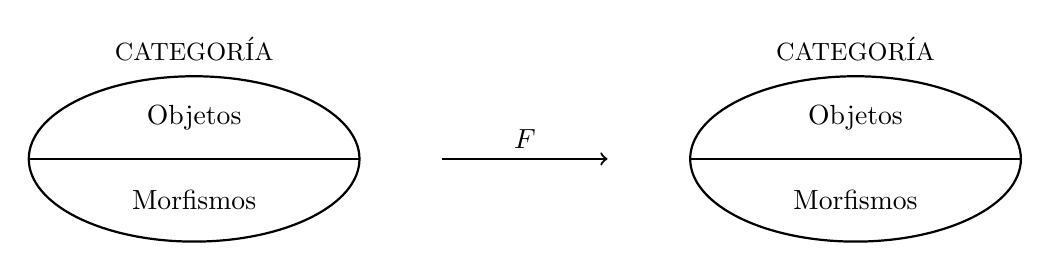
\begin{tikzpicture}[scale=0.7]
				% Categoría izquierda
				\begin{scope}[shift={(-6,0)}]
					\draw[thick] (0,0) ellipse (3cm and 1.5cm);
					\draw[thick] (-3,0) -- (3,0);
					\node at (0,2) {{\small CATEGORÍA}};
					\node at (0,0.75) {Objetos};
					\node at (0,-0.75) {Morfismos};
				\end{scope}
				
				% Categoría derecha
				\begin{scope}[shift={(6,0)}]
					\draw[thick] (0,0) ellipse (3cm and 1.5cm);
					\draw[thick] (-3,0) -- (3,0);
					\node at (0,2) {{\small CATEGORÍA}};
					\node at (0,0.75) {Objetos};
					\node at (0,-0.75) {Morfismos};
				\end{scope}
				
				% Flecha
				\draw[->, thick] ( -1.5, 0 ) -- ( 1.5, 0 ) node[midway, above] {\(F\)};
			\end{tikzpicture}
		\end{center}
		
		\noindent A todo objeto $A$ de la primera categoría se le hace corresponder un único objeto $F(A)$ de la segunda categoría, y a cada morfismo $f$ se le hace corresponder un único morfismo $F(f)$, preservando identidad y composición.
	}
\end{observacion}



\begin{definicion}
	\upshape{
		La \textit{categoría opuesta} de una categoría $\mathcal{C}$ se denota por $\mathcal{C}^{\mathrm{op}}$ y se define de la siguiente manera:
		
		\begin{enumerate}
			\item Los objetos de $\mathcal{C}^{\mathrm{op}}$ son los mismos que los de $\mathcal{C}$:
			$$
			\mathrm{Ob}(\mathcal{C}^{\mathrm{op}}) := \mathrm{Ob}(\mathcal{C}).
			$$
			
			\item Dados dos objetos $A$ y $B$, el conjunto de morfismos de $A$ a $B$ en $\mathcal{C}^{\mathrm{op}}$ se define como
			$$
			\mathrm{Hom}_{\mathcal{C}^{\mathrm{op}}}(A, B) := \mathrm{Hom}_{\mathcal{C}}(B, A).
			$$
			Es decir, un morfismo $f \in \mathrm{Hom}_{\mathcal{C}}(B, A)$ se considera en $\mathcal{C}^{\mathrm{op}}$ como un morfismo de $A$ a $B$. Aunque se trata del mismo símbolo $f$, se interpreta con dirección opuesta.
			
			\item La composición de morfismos en $\mathcal{C}^{\mathrm{op}}$ se define por
			$$
			f^{\mathrm{op}} \circ g^{\mathrm{op}} := (g \circ f)^{\mathrm{op}},
			$$
			donde $f \in \mathrm{Hom}_{\mathcal{C}}(B, C)$ y $g \in \mathrm{Hom}_{\mathcal{C}}(A, B)$. Esto garantiza que la composición en $\mathcal{C}^{\mathrm{op}}$ corresponde a la composición en $\mathcal{C}$ pero en orden inverso.
			
			\item Para cada objeto $A$, el morfismo identidad en $\mathcal{C}^{\mathrm{op}}$ es el mismo que en $\mathcal{C}$:
			$$
			\mathrm{id}_A^{\mathrm{op}} := \mathrm{id}_A.
			$$
			
			\item La composición en $\mathcal{C}^{\mathrm{op}}$ es asociativa, ya que la composición en $\mathcal{C}$ lo es.
		\end{enumerate}
	}
\end{definicion}






\begin{observacion}
	\upshape{
		Si $F: \mathcal{C}^{\mathrm{op}} \to \mathcal{D}$ es un functor, entonces para todo par de  morfismos $f: A \to B$ y $g: B \to C$ en $\mathcal{C}$, se tiene
		$$
		F(g \circ f) = F(f) \circ F(g).
		$$
		Es decir, $F$ invierte el orden de la composición.
	}
\end{observacion}

\begin{proof}[Justificación]
	Dado que en $\mathcal{C}^{\mathrm{op}}$ el morfismo \( f: A \to B \) en $\mathcal{C}$ se interpreta como \( f: B \to A \), y análogamente \( g: B \to C \) como \( g: C \to B \), en $\mathcal{C}^{\mathrm{op}}$ se tiene
	$$
	f: B \to A, \quad g: C \to B, \quad \text{de modo que } f \circ g: C \to A,
	$$
	lo cual, por definición de composición en $\mathcal{C}^{\mathrm{op}}$, corresponde a \( g \circ f \) en $\mathcal{C}$. Entonces, como \(F\) es un functor, se aplica
	$$ F(f \circ g) = F(f) \circ F(g), $$
	y al identificar \( f \circ g \) en $\mathcal{C}^{\mathrm{op}}$ con \( g \circ f \) en $\mathcal{C}$, se concluye
	$$F(g \circ f) = F(f) \circ F(g). $$
	
	\noindent Esto se ilustra en el siguiente diagrama conmutativo:
	
	$$
	{\Large
		\xymatrix{
			A \ar[rr]^f \ar[ddrr]_{g\circ f}& & B \ar[dd]^g &          &  & F(A)  & & F(B) \ar[ll]_{F(f)}  \\
			& &             & \ar[rr]^F &  &                                            & &\\
			& & C           &          &  &                                            & &  F(C)  \ar[uull]^{F(g\circ f)} \ar[uu]_{F(g)}
		}
	} 
	$$
	
\end{proof}

\begin{definicion}
	\upshape{
		Sean $\mathcal{C}$ y $\mathcal{D}$ dos categorías. Según el dominio de definición, distinguimos dos tipos de functores:
		\begin{enumerate}
			\item Un \textit{functor covariante} es un functor $F: \mathcal{C} \to \mathcal{D}$.
			\item Un \textit{functor contravariante} es un functor $F: \mathcal{C}^{\mathrm{op}} \to \mathcal{D}$, el cual se suele interpretar como una asignación
			$$
			F: \mathcal{C} \to \mathcal{D}
			$$
			que invierte la dirección de los morfismos.
		\end{enumerate}
	}
\end{definicion}





\begin{ejemplo}[Functor dual]\label{ejemplofunctor dual}
	\upshape{
		Sea $\mathbf{Vect}_{\mathbb{K}}$ la categoría de espacios vectoriales sobre un cuerpo $\mathbb{K}$.
		
		\begin{itemize}
			\item Para todo espacio vectorial $V$, se define su \textit{espacio dual} como $V^* := \mathrm{Hom}_{\mathbb{K}}(V, \mathbb{K}),$
			el conjunto de transformaciones lineales de $V$ en $\mathbb{K}$.
			
			\item Si $f: V \to W$ es una transformación lineal, se define su \textit{transformación dual} como $
			f^*: W^* \to V^*, \quad \phi \mapsto \phi \circ f,$ que es lineal.
		\end{itemize}
		Estas asignaciones definen el functor dual
		
		\begin{align*}
			F : \mathbf{Vect}_{\mathbb{K}}^{\mathrm{op}}& \longrightarrow \mathbf{Vect}_{\mathbb{K}}\\[5pt]
			V&\longmapsto V^\ast\\
			\left(f: V\to W \text{ en } \mathbf{Vect}_{\mathbb{K}}\right)&\longmapsto \left(f^\ast: W^\ast \to V^\ast\right).
		\end{align*}
		Es decir, a cada espacio $V$ le asigna su dual $V^*$, y a cada morfismo $f$ su dual $f^*$.\\
		
		
		\noindent Para verificar que $F$ define un functor $F: \textbf{Vect}^{\mathrm{op}} \to \textbf{Vect}$, seguimos los pasos de la definición:
		
		\begin{enumerate}
			\item Asignación sobre objetos:
			A cada objeto $V \in \mathrm{Ob}(\textbf{Vect}^{\mathrm{op}}) = \mathrm{Ob}(\textbf{Vect})$, el functor $F$ le asigna su dual $V^* = \mathrm{Hom}_{\textbf{Vect}}(V, \mathbb{K})$, que también es un espacio vectorial sobre $\mathbb{K}$. Por tanto, $F(V) \in \mathrm{Ob}(\textbf{Vect})$.
			
			\item Asignación sobre morfismos:
			A cada morfismo $f \in \mathrm{Hom}_{\textbf{Vect}^{\mathrm{op}}}(V, W)$, esto significa, $f: W \to V$ en $\textbf{Vect}$, el functor $F$ le asigna
			$$
			F(f) = f^* : V^* \to W^*, \quad \phi \mapsto \phi \circ f,
			$$
			que es un morfismo lineal entre espacios vectoriales.
			
			\item Preserva la identidad: Para todo espacio vectorial $V$,
			$$
			F(\mathrm{id}_V) = (\mathrm{id}_V)^* : V^* \to V^*, \quad \phi \mapsto \phi \circ \mathrm{id}_V = \phi,
			$$
			que es la identidad en $V^*$.
			
			\item Preserva la composición: Dados $f: V \to W$ y $g: W \to X$,
			$$
			F(g \circ f) = (g \circ f)^* : X^* \to V^*, \quad \phi \mapsto \phi \circ (g \circ f),
			$$
			mientras que
			$$
			F(f) \circ F(g) = f^* \circ g^* : X^* \to V^*, \quad \phi \mapsto f^*(g^*(\phi)) = f^*(\phi \circ g) = (\phi \circ g) \circ f = \phi \circ (g \circ f).
			$$
			Por lo tanto, $F(g \circ f) = F(f) \circ F(g)$.
		\end{enumerate}
		
		\noindent
		Con esto se concluye que $F$ es un functor de $\textbf{Vect}$ a sí misma.
		
	}
\end{ejemplo}

\begin{observacion}
	\upshape{
	En el Ejemplo \ref{ejemplofunctor dual} el functor dual es un functor contravariante.
	}
\end{observacion}
\begin{observacion}
	\upshape{
		Al definir un functor \( F \) desde \( \textbf{Vect}^{\mathrm{op}} \) en lugar de desde \( \textbf{Vect} \), se garantiza que la dirección de los morfismos sea compatible con la construcción dual. En efecto, una aplicación lineal \( f: V \to W \) induce naturalmente un morfismo \( f^*: W^* \to V^* \), que va en la dirección opuesta. Para que \( F \) sea un functor, se requiere que asigne a cada \( f \in \mathrm{Hom}_{\textbf{Vect}^{\mathrm{op}}}(V,W) \) un morfismo \( F(f) \in \mathrm{Hom}(F(V), F(W)) \), es decir, un morfismo de \( V^* \) en \( W^* \). Esto se logra al tomar como categoría de partida a \( \textbf{Vect}^{\mathrm{op}} \), de modo que el morfismo \( f: V \to W \) en \( \textbf{Vect} \) se interprete como un morfismo \( f: W \to V \) en \( \textbf{Vect}^{\mathrm{op}} \), y así \( f^*: V^* \to W^* \) encaje en la dirección correcta.
	}
\end{observacion}
  



\begin{ejemplo}[Functor bidual]\label{functorbidual}
	\upshape{
		Sea $\mathbf{Vect}_{\mathbb{K}}$ la categoría de espacios vectoriales sobre un cuerpo $\mathbb{K}$.
		
		\begin{itemize}
			\item Para cada espacio vectorial $V$, se define su \textit{bidual} como $V^{**} := (V^*)^*$, es decir, el dual del espacio dual de $V$.
			
			\item Dada una transformación lineal $f: V \to W$, su transformación bidual es
			$$
			f^{**} : V^{**} \to W^{**}, \quad \Psi \mapsto f^{**}(\Psi),
			$$
			donde $f^{**}(\Psi)$ es la aplicación lineal en $W^*$ dada por
			$$
			f^{**}(\Psi)(\phi) :=\left(\Psi\circ f^\ast\right)(\phi)= \Psi(\phi \circ f), \quad \text{para toda } \phi \in W^*.
			$$
			Esto es, $f^{**}$ se define como la dual de la aplicación dual \( f^* : W^* \to V^* \).
		\end{itemize}
		
		Estas asignaciones definen un functor
		\begin{align*}
			F : \mathbf{Vect}_{\mathbb{K}} &\longrightarrow \mathbf{Vect}_{\mathbb{K}}\\[5pt]
			V &\longmapsto V^{**}\\
			\left(f: V \to W\right) &\longmapsto \left(f^{**} : V^{**} \to W^{**}\right).
		\end{align*}
		
		\noindent Verifiquemos que $F$ define un functor:
		
		\begin{enumerate}
			\item Asignación sobre objetos: A cada espacio $V$, el functor $F$ le asigna su bidual $V^{**}$.
			
			\item Asignación sobre morfismos: A cada morfismo $f: V \to W$, se le asigna $f^{**} : V^{**} \to W^{**}$ como se definió arriba.
			
			\item Preserva la identidad: Para todo $V$,
			$$
			F(\mathrm{id}_V) = (\mathrm{id}_V)^{**} = \mathrm{id}_{V^{**}}.
			$$
			
			\item Preserva la composición: Dados $f: V \to W$ y $g: W \to X$, se tiene
			$$
			F(g \circ f) = (g \circ f)^{**} = g^{**} \circ f^{**} = F(g) \circ F(f).
			$$
		\end{enumerate}
		
		\noindent
		Por lo tanto, $F$ es un functor de $\mathbf{Vect}_{\mathbb{K}}$.
	}
\end{ejemplo}

\begin{observacion}
	\upshape{
		En el Ejemplo \ref{functorbidual} el functor dual es un functor covariante.
	}
\end{observacion}


\begin{ejemplo}[Functor olvidadizo]
	\upshape{
		En teoría de categorías, un \textit{functor olvidadizo} es un functor que “olvida” parte de la estructura o propiedades de los objetos y morfismos de una categoría para considerarlos en una categoría más simple. Por ejemplo, al pasar de espacios vectoriales a conjuntos, se olvida la estructura vectorial y se conserva únicamente la información del conjunto subyacente.\\
		
		\noindent Sea $\mathbf{Vect}_{\mathbb{K}}$ la categoría de espacios vectoriales sobre un cuerpo $\mathbb{K}$ y $\mathbf{Set}$ la categoría de conjuntos.
		
		\begin{itemize}
			\item A cada espacio vectorial $V$, el functor olvidadizo $F$ le asigna el conjunto subyacente de vectores de $V$.
			
			\item A cada transformación lineal $f: V \to W$, el functor le asigna la misma función $f$ vista como función entre conjuntos.
		\end{itemize} Así, el functor olvidadizo se define como
		\begin{align*}
			F : \mathbf{Vect}_{\mathbb{K}} &\longrightarrow \mathbf{Set}\\[5pt]
			V &\longmapsto F(V)\\
			(f: V \to W) &\longmapsto F(f).
		\end{align*}
		
		\noindent	Verificación de que $F$ es un functor:
		\begin{enumerate}
			\item Preserva la identidad: Para todo espacio vectorial $V$,
			$$
			F(\mathrm{id}_V) = \mathrm{id}_{F(V)}.
			$$
			
			\item Preserva la composición: Dados morfismos $f: V \to W$ y $g: W \to X$,
			$$
			F(g \circ f) = g \circ f = F(g) \circ F(f).
			$$
		\end{enumerate}
		
		Por lo tanto, $F$ es un functor de $\mathbf{Vect}_{\mathbb{K}}$ a $\mathbf{Set}$, llamado \textit{functor olvidadizo}.
	}
\end{ejemplo}



\begin{ejemplo}[Otros functores olvidadizos]
	\upshape{
		A continuación se muestran varios ejemplos de functores olvidadizos, indicando explícitamente su acción en objetos y morfismos mediante \texttt{align*}:
		
		\begin{itemize}
			\item De $\mathbf{Top}$ a $\mathbf{Set}$: \\
			El functor olvidadizo que asigna a cada espacio topológico su conjunto subyacente y a cada función continua la misma función vista como mapeo de conjuntos.
			\begin{align*}
				F : \mathbf{Top} &\longrightarrow \mathbf{Set}\\[5pt]
				(X, \tau) &\longmapsto X\\
				(f: X \to Y) &\longmapsto f: X \to Y.
			\end{align*}
			
			\item De $\mathbf{Vect}_{\mathbb{K}}^{\|\cdot\|}$ a $\mathbf{Top}$: \\
			El functor olvidadizo que a cada espacio vectorial normado le asigna el espacio topológico subyacente (con la topología inducida por la norma), y a cada transformación lineal continua la misma función.
			\begin{align*}
				F : \mathbf{Vect}_{\mathbb{K}}^{\|\cdot\|} &\longrightarrow \mathbf{Top}\\[5pt]
				(V, \|\cdot\|) &\longmapsto (V, \text{topología inducida por } \|\cdot\|)\\
				(f: V \to W,\ f\ \text{continua}) &\longmapsto f: V \to W.
			\end{align*}
			
			\item De $\mathbf{Vect}_{\mathbb{K}}^{\|\cdot\|}$ a $\mathbf{Vect}_{\mathbb{K}}$: \\
			El functor olvidadizo que “olvida” la norma, asignando a cada espacio vectorial normado su espacio vectorial subyacente y a cada transformación lineal continua la misma transformación lineal en $\mathbf{Vect}_{\mathbb{K}}$.
			\begin{align*}
				F : \mathbf{Vect}_{\mathbb{K}}^{\|\cdot\|} &\longrightarrow \mathbf{Vect}_{\mathbb{K}}\\[5pt]
				(V, \|\cdot\|) &\longmapsto V\\
				(f: V \to W,\ f\ \text{continua}) &\longmapsto f: V \to W.
			\end{align*}
			
			\item De $\mathbf{Grp}$ a $\mathbf{Set}$: \\
			El functor olvidadizo que asigna a cada grupo su conjunto subyacente y a cada homomorfismo de grupos la misma función vista como función de conjuntos.
			\begin{align*}
				F : \mathbf{Grp} &\longrightarrow \mathbf{Set}\\[5pt]
				G &\longmapsto G\\
				(\varphi: G \to H) &\longmapsto \varphi: G \to H.
			\end{align*}
			
			\item De $\mathbf{Ring}$ a $\mathbf{Ab}$: \\
			El functor olvidadizo que asigna a cada anillo su grupo aditivo subyacente y a cada homomorfismo de anillos la misma función como homomorfismo de grupos abelianos.
			\begin{align*}
				F : \mathbf{Ring} &\longrightarrow \mathbf{Ab}\\[5pt]
				(R, +, \cdot) &\longmapsto (R, +)\\
				(\psi: R \to S) &\longmapsto \psi: (R, +) \to (S, +).
			\end{align*}
		\end{itemize}
	}
\end{ejemplo}


\begin{ejemplo}[Functor Hom covariante]\label{functorhom}
	\upshape{
		Sean $\mathcal{C}$ una categoría y $A \in \mathrm{Ob}(\mathcal{C})$ un objeto fijo. Consideremos las siguientes construcciones:
		
		\begin{itemize}
			\item Para cada objeto $X \in \mathcal{C}$, se asocia el conjunto $\mathrm{Hom}_{\mathcal{C}}(A, X)$.
			
			\item Para cada morfismo $f : X \to Y$ en $\mathcal{C}$, se define la función
			\[
			\mathrm{Hom}_{\mathcal{C}}(A, f) : \mathrm{Hom}_{\mathcal{C}}(A, X) \to \mathrm{Hom}_{\mathcal{C}}(A, Y), \quad h \mapsto f \circ h.
			\]
		\end{itemize}
		
		Estas asignaciones definen un functor
		\begin{align*}
			\mathrm{Hom}_{\mathcal{C}}(A, -) : \mathcal{C} &\longrightarrow \mathbf{Set}\\[5pt]
			X &\longmapsto \mathrm{Hom}_{\mathcal{C}}(A, X)\\
			(f : X \to Y) &\longmapsto \left(\mathrm{Hom}_{\mathcal{C}}(A, f) : \mathrm{Hom}_{\mathcal{C}}(A, X) \to \mathrm{Hom}_{\mathcal{C}}(A, Y)\right).
		\end{align*}
		
		\noindent Verifiquemos que esta asignación define un functor:
		
		\begin{enumerate}
			\item Asignación sobre objetos: A cada objeto $X$ de $\mathcal{C}$, se le asigna el conjunto $\mathrm{Hom}_{\mathcal{C}}(A, X)$.
			
			\item Asignación sobre morfismos: A cada morfismo $f : X \to Y$, se le asigna la función $\mathrm{Hom}_{\mathcal{C}}(A, f)$ dada por la composición a derecha con $f$.
			
			\item Preserva la identidad: Para todo objeto $X$, se tiene
			\[
			\mathrm{Hom}_{\mathcal{C}}(A, \mathrm{id}_X)(h) = \mathrm{id}_X \circ h = h,
			\]
			para todo $h \in \mathrm{Hom}_{\mathcal{C}}(A, X)$, es decir,
			\[
			\mathrm{Hom}_{\mathcal{C}}(A, \mathrm{id}_X) = \mathrm{id}_{\mathrm{Hom}_{\mathcal{C}}(A, X)}.
			\]
			
			\item Preserva la composición: Dado $f : X \to Y$ y $g : Y \to Z$ en $\mathcal{C}$, se tiene que para todo $h \in \mathrm{Hom}_{\mathcal{C}}(A, X)$,
			\[
			\mathrm{Hom}_{\mathcal{C}}(A, g \circ f)(h) = (g \circ f) \circ h = g \circ (f \circ h) = \mathrm{Hom}_{\mathcal{C}}(A, g)(\mathrm{Hom}_{\mathcal{C}}(A, f)(h)).
			\]
			Así,
			\[
			\mathrm{Hom}_{\mathcal{C}}(A, g \circ f) = \mathrm{Hom}_{\mathcal{C}}(A, g) \circ \mathrm{Hom}_{\mathcal{C}}(A, f).
			\]
		\end{enumerate}
		
		\noindent
		Por lo tanto, $\mathrm{Hom}_{\mathcal{C}}(A, -)$ define un functor covariante de $\mathcal{C}$ a $\mathbf{Set}$.
	}
\end{ejemplo}
\begin{observacion}[Functor Hom contravariante]
	\upshape{
		De manera análoga al Ejemplo \ref{functorhom}, se puede fijar un objeto \( A \in \mathrm{Ob}(\mathcal{C}) \) y considerar la asignación
		\begin{align*}
			\mathrm{Hom}_{\mathcal{C}}(-, A) : \mathcal{C}^{\mathrm{op}} &\longrightarrow \mathbf{Set}\\[5pt]
			X &\longmapsto \mathrm{Hom}_{\mathcal{C}}(X, A)\\
			(f : X \to Y) &\longmapsto \left(\mathrm{Hom}_{\mathcal{C}}(f, A) : \mathrm{Hom}_{\mathcal{C}}(Y, A) \to \mathrm{Hom}_{\mathcal{C}}(X, A)\right),
		\end{align*}
		donde \( \mathrm{Hom}_{\mathcal{C}}(f, A)(h) = h \circ f \). \\
		
		\noindent Esta asignación define un functor contravariante \( \mathrm{Hom}_{\mathcal{C}}(-, A) \) de \( \mathcal{C} \) a \( \mathbf{Set} \), ya que:
		\begin{itemize}
			\item Preserva identidades: \( \mathrm{Hom}_{\mathcal{C}}(\mathrm{id}_X, A)(h) = h \circ \mathrm{id}_X = h \), para todo \( h \in \mathrm{Hom}_{\mathcal{C}}(X, A) \).
			
			\item Invierte la composición: dados \( f : X \to Y \) y \( g : Y \to Z \), se tiene
			\[
			\mathrm{Hom}_{\mathcal{C}}(g \circ f, A)(h) = h \circ (g \circ f) = (h \circ g) \circ f = \mathrm{Hom}_{\mathcal{C}}(f, A)(\mathrm{Hom}_{\mathcal{C}}(g, A)(h)),
			\]
			por lo que
			\[
			\mathrm{Hom}_{\mathcal{C}}(g \circ f, A) = \mathrm{Hom}_{\mathcal{C}}(f, A) \circ \mathrm{Hom}_{\mathcal{C}}(g, A).
			\]
		\end{itemize}
		
		\noindent
		Por lo tanto, \( \mathrm{Hom}_{\mathcal{C}}(-, A) \) es un functor contravariante de \( \mathcal{C} \) a \( \mathbf{Set} \), o equivalentemente, un functor covariante \( \mathcal{C}^{\mathrm{op}} \to \mathbf{Set} \).
	}
\end{observacion}


\section{Transformaciones naturales}

\begin{definicion}
	\upshape{
		Sean $\mathcal{C}$ y $\mathcal{D}$ dos categorías y $F, G: \mathcal{C} \to \mathcal{D}$ dos functores. Una \emph{transformación natural}
		$$
		\Phi: F \Longrightarrow G
		$$
		es una familia de morfismos 
		$$
		\{\Phi_A: F(A)\to G(A)\}_{\,A\in\mathrm{Ob}(\mathcal{C})\!}
		$$
		en $\mathcal{D}$ que satisface la siguiente condición: para todo morfismo $f: A\to B$ en $\mathcal{C}$, el diagrama
		
		$$
		{\Large 
			\xymatrix{
				F(A) \ar[rr]^{\Phi_A} \ar[dd]_{F(f)} && G(A) \ar[dd]^{G(f)} \\ \\
				F(B) \ar[rr]_{\Phi_B} && G(B)
			}
		}
		$$
		
	\noindent	conmuta, es decir,
		$G(f)\,\circ\,\Phi_A \;=\; \Phi_B\,\circ\,F(f).$\\
		
		\noindent Cada $\Phi_A$ se denomina \textit{componente} de $\Phi$ en $A$.
	}
\end{definicion}


\begin{ejemplo}\label{cascas}
	\upshape{
		Sean $\mathcal{C}$ y $\mathcal{D}$ dos categorías, y sea $F : \mathcal{C} \longrightarrow \mathcal{D}$ un functor. Definimos una transformación natural 
		$$
		\mathrm{id}_F : F \Longrightarrow F
		$$
		mediante la familia de morfismos 
		$$
		\bigl\{\, (\mathrm{id}_F)_A := \mathrm{id}_{F(A)} : F(A) \to F(A) \,\bigr\}_{\,A \in \mathrm{Ob}(\mathcal{C})}.
		$$
		Para verificar que $\mathrm{id}_F$ es natural, tomemos un morfismo arbitrario
		$f : A \longrightarrow B
		$ en $\mathcal{C}$. Debemos comprobar que el siguiente diagrama conmuta:
		$$
		{\large \xymatrix{
				F(A) \ar[rrr]^{(\mathrm{id}_F)_A} \ar[dd]_{F(f)} &&& F(A) \ar[dd]^{F(f)} \\
				&&& \\
				F(B) \ar[rrr]_{(\mathrm{id}_F)_B} &&& F(B)
		}}
		$$
		En efecto, se tiene:
		$$
		F(f) \circ (\mathrm{id}_F)_A = F(f) \circ \mathrm{id}_{F(A)} = F(f),
		$$
		y
		$$
		(\mathrm{id}_F)_B \circ F(f) = \mathrm{id}_{F(B)} \circ F(f) = F(f),
		$$
		por lo tanto,
		$$
		F(f) \circ (\mathrm{id}_F)_A = (\mathrm{id}_F)_B \circ F(f).
		$$
		Esto muestra que 
		$	\mathrm{id}_F : F \Longrightarrow F$ es una transformación natural.
	}
\end{ejemplo}




\begin{ejemplo}
	\upshape{
		En la categoría $\mathbf{Vect}_{\mathbb{K}}$, consideremos:
		\begin{itemize}
			\item El functor identidad 
			$$
			\mathrm{id}: \mathbf{Vect}_{\mathbb{K}}\longrightarrow \mathbf{Vect}_{\mathbb{K}},\quad V\longmapsto V,
			$$
			\item  El functor bidual 
			$$
			(-)^{**}: \mathbf{Vect}_{\mathbb{K}}\longrightarrow \mathbf{Vect}_{\mathbb{K}},\quad V\longmapsto V^{**}.
			$$
		\end{itemize}
		Definimos una transformación natural 
		$$
		\Phi: \mathrm{id} \Longrightarrow (-)^{**}
		$$
		mediante la familia de morfismos 
		$$
		\{\Phi_V : V \to V^{**}\}_{\,V\in\mathrm{Ob}(\mathbf{Vect}_{\mathbb{K}})} 
		$$
		donde, para cada espacio vectorial $V$, definimos el morfismo
		$$
		\Phi_V(v) \;:=\; \bigl[\;\phi \mapsto \phi(v)\bigr]\quad\text{para todo }v\in V,\;\phi\in V^*.
		$$
		
		\noindent Para verificar que $\Phi$ es natural, tomemos una transformación lineal 
		$$
		f: V \longrightarrow W,
		$$
		y debemos comprobar que el siguiente diagrama conmuta:
		$$
		{\Large \xymatrix{
			V \ar[rrr]^{\Phi_V} \ar[dd]_{f} && & V^{**} \ar[dd]^{f^{**}} \\
			&&&\\
			W \ar[rrr]_{\Phi_W} & && W^{**}
		}}
		$$
		En efecto, para cada $v\in V$ y cada $\psi\in W^*$, se tiene
		$$
		(f^{**}\circ \Phi_V)(v) \;=\; f^{**}(\Phi_V(v))
		\;=\; f^{**}\bigl[\;\phi\mapsto \phi(v)\bigr]
		\;=\; \bigl[\;\psi\mapsto \Phi_V(v)(\psi\circ f)\bigr]
		\;=\; \bigl[\;\psi\mapsto \psi(f(v))\bigr],
		$$
		y
		$$
		(\Phi_W\circ f)(v) \;=\; \Phi_W(f(v))
		\;=\; \bigl[\;\psi\mapsto \psi(f(v))\bigr].
		$$
		Por lo tanto,
		$$
		f^{**}\circ \Phi_V \;=\; \Phi_W\circ f,
		$$
		y el diagrama conmuta para todo $f$. Esto muestra que 
		$$
		\Phi: \mathrm{id} \Longrightarrow (-)^{**}
		$$
		es una transformación natural en $\mathbf{Vect}_{\mathbb{K}}$.
	}
\end{ejemplo}


\begin{ejemplo}
	\upshape{
		En la categoría \(\mathbf{Vect}_{\mathbb{K}}\), consideremos los siguientes functores:
		\begin{itemize}
			\item El functor identidad:
			\[
			\mathrm{id}: \mathbf{Vect}_{\mathbb{K}} \longrightarrow \mathbf{Vect}_{\mathbb{K}}, \quad V \longmapsto V,
			\]
			\item El functor bidual, revisar el Ejemplo \ref{functorbidual}:
			\[
			(-)^{**}: \mathbf{Vect}_{\mathbb{K}} \longrightarrow \mathbf{Vect}_{\mathbb{K}}, \quad V \longmapsto V^{**}.
			\]
		\end{itemize}
		Recordemos que todo vector \(v \in V\) define de manera natural un funcional sobre \(V^*\), dado por:
		$\phi \longmapsto \phi(v), \quad \text{para todo } \phi \in V^*$.
		Esto induce un morfismo lineal:
	
		\begin{align*}
			\Phi_V: V &\longrightarrow V^{**}\\
			v &\longmapsto 
			\left(
			\begin{array}{rcl}
				\Phi_V(v)\colon & V^* & \to \mathbb{K} \\
				& \phi & \mapsto \phi(v)
			\end{array}
			\right)
		\end{align*}
		De esta forma, definimos una transformación natural:
		$$
		\Phi: \mathrm{id} \Longrightarrow (-)^{**},
		$$
		dada por la familia de morfismos
		$$
		\left\{\, \Phi_V: V \to V^{**} \,\right\}_{V \in \mathrm{Ob}(\mathbf{Vect}_{\mathbb{K}})}.
		$$		
		Para verificar que \(\Phi\) es natural, tomemos una transformación lineal $
		f: V \longrightarrow W$,
		y comprobemos que el siguiente diagrama conmuta:
		$$
		{\Large \xymatrix{
				V \ar[rrr]^{\Phi_V} \ar[dd]_{f} &&& V^{**} \ar[dd]^{f^{**}} \\
				\\
				W \ar[rrr]_{\Phi_W} &&& W^{**}
		}}
		$$
		En efecto, para cada $v \in V$ y cada $\psi \in W^*$, se tiene: $$(f^{**} \circ \Phi_V)(v)
		= f^{\ast\ast}\left(\Phi_V(v)\right)=\Phi_V(v)\circ f^\ast ,$$ de donde se tiene $$(f^{**} \circ \Phi_V)(v)
		(\psi)=\Phi_V(v) \left(f^{\ast}(\psi)\right)=\Phi_V(v) \left(\psi \circ f\right)=\left(\psi \circ f\right)(v)$$
		y por otro lado:
		$$
		(\Phi_W \circ f)(v)(\psi) = \Phi_W(f(v))(\psi) = \psi(f(v)).
		$$
		Por lo tanto,
		\[
		f^{**} \circ \Phi_V = \Phi_W \circ f,
		\]
		y el diagrama conmuta para todo \(f\).
	}
\end{ejemplo}

\begin{definicion}
	\upshape{
		Sean \(\mathcal{C}\) y \(\mathcal{D}\) categorías, y \(F, G, H : \mathcal{C} \to \mathcal{D}\) tres functores. Y sean \(\Phi : F \Longrightarrow G\) y \(\Psi : G \Longrightarrow H\) transformaciones naturales. La \emph{composición} de \(\Phi\) con \(\Psi\), denotada por $\Psi \circ \Phi$ está definida para cada objeto \(A \in \mathcal{C}\) por
		$$
		(\Psi \circ \Phi)_A := \Psi_A \circ \Phi_A: F(A) \to H(A).
		$$ 		Así, la composición de transformaciones naturales se obtiene componiendo las componentes en cada objeto.
	}
\end{definicion}

\begin{proposicion}\label{lkjhgf}
	\upshape{
		La composición de transformaciones naturales es una transformación natural.
	}
\end{proposicion}

\begin{proof}
	Sea \(\mathcal{C}\) y \(\mathcal{D}\) dos categorías, y \(F, G, H : \mathcal{C} \to \mathcal{D}\) tres functores. Sean 
	\[
	\Phi : F \Longrightarrow G, \quad \Psi : G \Longrightarrow H
	\]
	transformaciones naturales con componentes \(\{\Phi_A\}_{A \in \mathrm{Ob}(\mathcal{C})}\) y \(\{\Psi_A\}_{A \in \mathrm{Ob}(\mathcal{C})}\).\\
	
	
	\noindent Queremos demostrar que \(\Psi \circ \Phi\) es una transformación natural, es decir, que para todo morfismo \(f : A \to B\) en \(\mathcal{C}\) el siguiente diagrama conmuta:
	\[
	{\Large
		\xymatrix{
			F(A) \ar[rr]^{(\Psi \circ \Phi)_A} \ar[dd]_{F(f)} && H(A) \ar[dd]^{H(f)} \\ \\
			F(B) \ar[rr]_{(\Psi \circ \Phi)_B} && H(B)
		}
	}
	\] Esto equivale a verificar que
	\[
	H(f) \circ (\Psi \circ \Phi)_A = (\Psi \circ \Phi)_B \circ F(f).
	\]	Por definición de composición,
	\[
	H(f) \circ \Psi_A \circ \Phi_A = \Psi_B \circ \Phi_B \circ F(f).
	\] Como \(\Psi\) es transformación natural,
	\[
	H(f) \circ \Psi_A = \Psi_B \circ G(f),
	\]
	y como \(\Phi\) es transformación natural,
	\[
	G(f) \circ \Phi_A = \Phi_B \circ F(f).
	\] Sustituyendo estas igualdades se obtiene:
	\[
	H(f) \circ \Psi_A \circ \Phi_A = \Psi_B \circ G(f) \circ \Phi_A = \Psi_B \circ \Phi_B \circ F(f).
	\] Por lo tanto, \(\Psi \circ \Phi\) es una transformación natural.
\end{proof}




\section{Functor de Yoneda}



\begin{proposicion}
	\upshape{
		Sean \( \mathcal{C} \) y \( \mathcal{D} \) categorías. Entonces, \( \mathcal{D}^\mathcal{C} \), cuya clase de objetos está formada por los functores \( F : \mathcal{C} \to \mathcal{D} \), y cuyos morfismos son las transformaciones naturales entre ellos, es una categoría.
	}
\end{proposicion}

\begin{proof}
	En efecto
	\begin{enumerate}
		
		\item \textbf{Objetos:} Son los functores \(F : \mathcal{C} \to \mathcal{D}\). Esto es $F\in \mathrm{Ob}\left(\mathcal{D}^\mathcal{C}\right)$.
		
		\item \textbf{Morfismos:} Son las transformaciones naturales, es decir, dados functores \(F, G : \mathcal{C} \to \mathcal{D}\), una transformación natural \(\Phi : F \Longrightarrow G\) es un morfismo, esto dignifica que, $\Phi \in \mathrm{Hom}_{\mathcal{D}^\mathcal{C}}(F,G)$
		
		\item \textbf{Composición:} Sean \(\Phi : F \Longrightarrow G\) y \(\Theta : G \Longrightarrow H\) transformaciones naturales. Por la Proposición \ref{lkjhgf} su composición \(\Theta \circ \Phi : F \Longrightarrow H\) es una transformación natural.
		
		\item \textbf{Identidad:} Para cada functor \(F\in \mathcal{D}^\mathcal{C}\), de Ejemlplo \ref{cascas}, existe la transformación natural identidad \(\mathrm{id}_F : F \Rightarrow F\). Verificamos cómo actúa respecto a la composición: \\
		
		\noindent Dado \(F \in \mathrm{Ob}(\mathcal{D}^\mathcal{C})\), sean \(G \in \mathrm{Ob}(\mathcal{D}^\mathcal{C})\), \(\Phi \in \mathrm{Hom}_{\mathcal{D}^\mathcal{C}}(F, G)\) y \(\Psi \in \mathrm{Hom}_{\mathcal{D}^\mathcal{C}}(G, F)\). Para cada objeto \(A \in \mathrm{Ob}(\mathcal{C})\), tenemos:
		\begin{align*}
			(\Phi \circ \mathrm{id}_F)_A &= \Phi_A \circ (\mathrm{id}_F)_A = \Phi_A \circ \mathrm{id}_{F(A)} = \Phi_A, \\
			(\mathrm{id}_F \circ \Psi)_A &= (\mathrm{id}_F)_A \circ \Psi_A = \mathrm{id}_{F(A)} \circ \Psi_A = \Psi_A.
		\end{align*}
		
		\noindent Por lo tanto,
		\[
		\Phi \circ \mathrm{id}_F = \Phi \quad \text{y} \quad \mathrm{id}_F \circ \Psi = \Psi.
		\]
	
		\item \textbf{Asociatividad:} Si \(\Phi : F \Rightarrow G\), \(\Theta : G \Rightarrow H\), \(\Psi : H \Rightarrow K\), entonces
		\[
		(\Psi \circ (\Theta \circ \Phi))_A = \Psi_A \circ (\Theta_A \circ \Phi_A) = (\Psi_A \circ \Theta_A) \circ \Phi_A = ((\Psi \circ \Theta) \circ \Phi)_A,
		\]
		por asociatividad de la composición en \(\mathcal{D}\). Luego,
		\[
		\Psi \circ (\Theta \circ \Phi) = (\Psi \circ \Theta) \circ \Phi.
		\]
	\end{enumerate}
\end{proof}
  
 
 

 
 
 
 
 
 
 \noindent Definimos 
 \begin{align*}
 	h : \mathcal{C} &\longrightarrow \mathbf{Set}^{\mathcal{C}^{\mathrm{op}}} \\
 	A &\longmapsto \mathrm{Hom}_{\mathcal{C}}(\,\_\,, A),\\
 	\left(f:A\to B\right)&\longmapsto \left( f^\ast: \mathrm{Hom}_{\mathcal{C}}(\_\,,A) \Longrightarrow \mathrm{Hom}_{\mathcal{C}}(\_\,,B)\right)
 \end{align*}
 donde 
 \begin{align*}
 	\mathrm{Hom}_{\mathcal{C}}(\,\_\,, A) : \mathcal{C}^{\mathrm{op}} &\longrightarrow \mathbf{Set} \\
 	X &\longmapsto \mathrm{Hom}_{\mathcal{C}}(X, A),
 \end{align*}
 y \(f^\ast\) está dada por la familia \(\left\{f^\ast_{X}: \mathrm{Hom}_{\mathcal{C}}(X,A)\to \mathrm{Hom}_{\mathcal{C}}(X,B)\right\}_{X \in \mathcal{C}}\), cuyas componentes se definen como
 \begin{align*}
 	f^\ast_X: \mathrm{Hom}_{\mathcal{C}}(X,A) &\longrightarrow \mathrm{Hom}_{\mathcal{C}}(X,B) \\
 	g &\longmapsto f \circ g.
 \end{align*}
 
 
 
 
 
 
 
 
 \noindent
 Para cada objeto \(A\) de \(\mathcal{C}\), denotamos por
 \[
 h_A := \mathrm{Hom}_{\mathcal{C}}(\_\,, A) : \mathcal{C}^{\mathrm{op}} \longrightarrow \mathbf{Set}.
 \]
 
 
 \begin{proposicion}
 	\upshape{
 		La asignación \(h : \mathcal{C} \to \mathbf{Set}^{\mathcal{C}^{\mathrm{op}}}\), dada por \(A \mapsto h_A\) y \(f \mapsto f^\ast\), define un functor covariante.
 	}
 \end{proposicion}
 
 
 
 
 \begin{proof}
 	Para demostrar que $h$ es un functor covariante, verificamos las siguientes propiedades:
 	\begin{enumerate}
 		
 		\item \textbf{Asignación a objetos:} Por definición, \( h(A) = h_A \in \mathbf{Set}^{\mathcal{C}^{\mathrm{op}}} \), ya que \( h_A \) es un functor contravariante de \( \mathcal{C} \) a \( \mathbf{Set} \).
 		
 		\item \textbf{Asignación a morfismos:} Dado \( f: A \to B \), definimos \( f^\ast: h_A \Longrightarrow h_B \) por \( f^\ast_X(g) := f \circ g \) para \( g \in \mathrm{Hom}_\mathcal{C}(X, A) \). Mostramos que esta es una transformación natural.\\
 		
 		\noindent Sea \( u: Y \to X \) en \( \mathcal{C}^{\mathrm{op}} \) (es decir, \( u: X \to Y \) en \( \mathcal{C} \)). Queremos probar que el siguiente diagrama conmuta:
 		
 		\[
 		\xymatrix @C=4.5em{
 			\mathrm{Hom}_\mathcal{C}(X, A) \ar[r]^{\displaystyle f^\ast_X} \ar[dd]_{\displaystyle h_A(u)} & \mathrm{Hom}_\mathcal{C}(X, B) \ar[dd]^{ \displaystyle h_B(u)} \\
 			&&\\
 			\mathrm{Hom}_\mathcal{C}(Y, A) \ar[r]_{ \displaystyle f^\ast_Y} & \mathrm{Hom}_\mathcal{C}(Y, B)
 		}
 		\]
 		
 		Para \( g \in \mathrm{Hom}_\mathcal{C}(X, A) \), tenemos:
 		\begin{align*}
 			(f^\ast_Y \circ h_A(u))(g) &= f^\ast_Y(g \circ u) && \text{(por definición de } h_A(u)\text{)} \\
 			&= f \circ (g \circ u) && \text{(por definición de } f^\ast_Y\text{)} \\
 			&= (f \circ g) \circ u && \text{(asociatividad)} \\
 			&= h_B(u)(f \circ g) && \text{(por definición de } h_B(u)\text{)} \\
 			&= (h_B(u) \circ f^\ast_X)(g) && \text{(por definición de } f^\ast_X\text{)}
 		\end{align*}
 		Así, \( f^\ast \) es una transformación natural.
 		
 		\item \textbf{Preservación de la composición:}
 		Sean $f: A \to B$ y $g: B \to C$ morfismos en $\mathcal{C}$. Debemos verificar que
 		\[
 		h(g \circ f) = h(g) \circ h(f),
 		\]
 		es decir, que
 		\[
 		(g \circ f)^\ast = g^\ast \circ f^\ast.
 		\]
 		Para cada objeto $X \in \mathcal{C}$ y cada $u \in \mathrm{Hom}_{\mathcal{C}}(X, A)$, tenemos:
 		\begin{align*}
 			((g \circ f)^\ast)_X(u) &= (g \circ f) \circ u && \text{(def. de } (g \circ f)^\ast_X) \\
 			&= g \circ (f \circ u) && \text{(asociatividad)} \\
 			&= g^\ast_X(f \circ u) && \text{(def. de } g^\ast_X) \\
 			&= g^\ast_X(f^\ast_X(u)) && \text{(def. de } f^\ast_X) \\
 			&= (g^\ast_X \circ f^\ast_X)(u) && \text{(composición de funciones)} \\
 			&= (g^\ast \circ f^\ast)_X(u) && \text{(def. de comp. de transf. nat.)}
 		\end{align*}
 		
 		\item \textbf{Preservación de identidades:}
 		Para cada objeto $A \in \mathcal{C}$, debemos verificar que
 		\[
 		h(\mathrm{id}_A) = \mathrm{id}_{h_A},
 		\]
 		es decir, que
 		\[
 		\mathrm{id}_A^\ast = \mathrm{id}_{h_A}.
 		\]
 		Para cada objeto $X \in \mathcal{C}$ y cada $g \in \mathrm{Hom}_{\mathcal{C}}(X, A)$:
 		\begin{align*}
 			(\mathrm{id}_A^\ast)_X(g) &= \mathrm{id}_A \circ g && \text{(por definición)} \\
 			&= g && \text{(identidad de la composición)} \\
 			&= (\mathrm{id}_{h_A})_X(g).
 		\end{align*}
 		Por lo tanto, $\mathrm{id}_A^\ast = \mathrm{id}_{h_A}$.
 		
 	\end{enumerate}
 	
 	Con esto, se concluye que \( h \) es un functor covariante.
 	
 
 \end{proof}
 
 
\begin{observacion}\upshape{
	
	Se utiliza la categoría opuesta \(\mathcal{C}^{\mathrm{op}}\) para definir \(h_A = \mathrm{Hom}_{\mathcal{C}}(\_, A)\) porque la variable donde actúa el morfismo en \(\mathrm{Hom}_{\mathcal{C}}(X, A)\) es contravariante. Es decir, un morfismo \(f: X \to Y\) induce una función \(\mathrm{Hom}_{\mathcal{C}}(Y, A) \to \mathrm{Hom}_{\mathcal{C}}(X, A)\) que va en dirección opuesta a \(f\). Por eso, para que \(h_A\) sea un functor covariante, consideramos los objetos y morfismos en \(\mathcal{C}^{\mathrm{op}}\), invirtiendo así las flechas y respetando la composición.
	}
\end{observacion}

 
\begin{definicion}
	\upshape{
		El \emph{functor de Yoneda} es el functor covariante
		\[
		h : \mathcal{C} \to \mathbf{Set}^{\mathcal{C}^\mathrm{op}},
		\]
		ya definido, que asigna a cada objeto \(A \in \mathcal{C}\) el functor  \(h_A = \mathrm{Hom}_{\mathcal{C}}(-, A)\) y a cada morfismo \(f: A \to B\) la transformación natural \(f^\ast : h_A \Longrightarrow h_B\).
	}
\end{definicion}


 
 
 
 